\chapter[Introdução]{Introdução}
  
  Será apresentado neste capítulo uma breve contextualização do negócio do Corpo de Bombeiros Militar do Distrito Federal.
  
  \section{Contexto do negócio}
  
  Ao nosso grupo foi atribuída a responsabilidade de propor a solução de \textit{software} para o Corpo de Bombeiros Militar
  do Distrito Federal (CBMDF), no que diz respeito ao gerenciamento de sua frota de veículos terrestre e afins.
  Para o melhor entendimento da solução proposta será explicado, de forma breve, alguns aspectos do CBMDF.
  
  O próprio lema do CBMDF nos resume a missão deles: “Vidas alheias e riquezas salvar” \cite{cbmdf12}.
  A fim de cumprir tal missão, possuem atribuições definidas em lei \cite{brasil09}: “O Corpo de Bombeiros Militar do Distrito
  Federal [...] destina-se à execução de serviços de perícia, prevenção e combate a incêndios, de busca e salvamento, e
  de atendimento pré-hospitalar e de prestação de socorros nos casos de sinistros, inundações, desabamentos, catástrofes,
  calamidades públicas e outros em que seja necessária a preservação da incolumidade das pessoas e do patrimônio.”.
  
  O CBMDF é um órgão público que integra o Sistema de Segurança Pública, sendo uma corporação militar possui uma caracterização
  militar muito forte em suas tradições, hábitos e hierarquia funcional, possuindo postos e graduações (vide Figura ~\ref{patentes_cbmdf}).
  Além disso, possui uma estrutura organizacional bastante hierárquica e estruturada em órgãos de direção, órgãos de apoio
  e órgãos de execução \cite{brasil91}. Tal definição é confirmada com a lei previamente mencionada, quando a mesma normatiza:
  “O Corpo de Bombeiros Militar do Distrito Federal, instituição […] fundamentada nos princípios da hierarquia e disciplina [...]”
  e a Figura ~\ref{organograma_simplificado_cbmdf} explicita. O regime militar, e a carreira pública inerente ao órgão, caracterizam um ambiente estável,
  pouco volátil e bastante formal.
  
  \begin{figure}[!htbp]
    \centering
    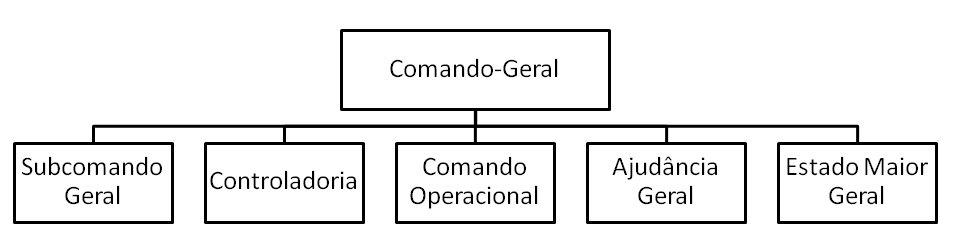
\includegraphics[scale=0.5]{editaveis/figuras/organograma_simplificado_cbmdf}
    \caption[Versão simplificada da estrutura organizacional do CBMDF]{Versão simplificada da estrutura organizacional do CBMDF. \footnotemark}
    \label{organograma_simplificado_cbmdf}
  \end{figure}
  \footnotetext{Baseada no organograma disponibilizado em <https://www.cbm.df.gov.br/portal2013/index.php?option=com\_edocman\&task=document.download\&id=2\&Itemid=144>.
  Acesso em 02/05/2015.}
  
  É valido lembrar que por se tratar de uma organização do setor público, além da estrutura hierárquica mencionada, alguns
  aspectos são inerentes e se aplicam fortemente, como regimentos, leis e demais normas, necessidade de licitações para prestação
  de serviços, etc.
  
  \begin{figure}[!htbp]
    \centering
    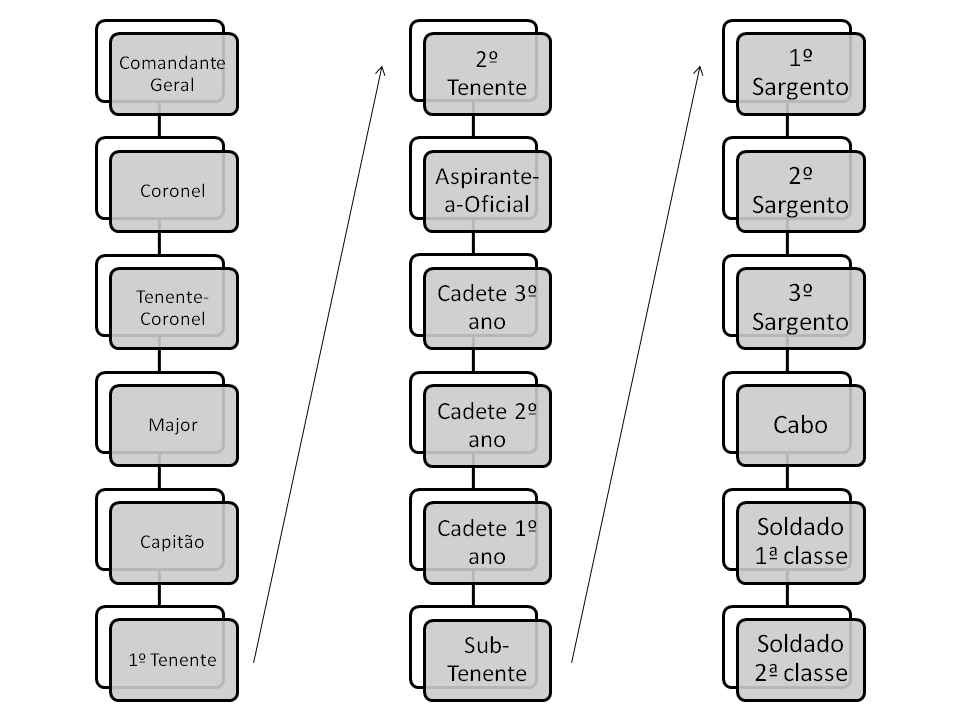
\includegraphics[scale=0.5]{editaveis/figuras/patentes_cbmdf}
    \caption[Postos e graduações do CBMDF]{Postos e graduações do CBMDF. \footnotemark}
    \label{patentes_cbmdf}
  \end{figure}
  \footnotetext{Baseado no texto disponibilizado em <https://www.cbm.df.gov.br/institucional/2012-11-13-16-52-15>. Acesso em 02/05/2015.}
  
  
  \vfill
  
  